\documentclass[aspectratio=169]{beamer}
\usetheme{Madrid}
\usecolortheme{default}
\usepackage[utf8]{inputenc}
\usepackage[T1]{fontenc}
\usepackage{booktabs}
\usepackage{graphicx}
\graphicspath{{../results/figures/}}

\title{k-Anonymity-Based Data Anonymization and Re-identification Risk Analysis}
\subtitle{MSCS 714 Data Privacy Seminar}
\author{Group Project}
\date{April 2026}

\begin{document}

\begin{frame}
    \titlepage
\end{frame}

\begin{frame}{Problem}
    \begin{itemize}
        \item Removing direct identifiers is not enough to prevent re-identification.
        \item Quasi-identifiers such as age, sex, education, occupation, and country can still enable linkage.
        \item We study how k-anonymity changes exact-match linkage risk and data utility.
    \end{itemize}
\end{frame}

\begin{frame}{Dataset}
    \begin{itemize}
        \item Adult Census Income dataset from UCI
        \item 32,561 rows and 15 columns
        \item Sensitive attribute: income (\texttt{>50K} vs \texttt{<=50K})
        \item QI Set A: age, sex, education, marital status
        \item QI Set B: age, sex, occupation, native country
    \end{itemize}
\end{frame}

\begin{frame}{Method}
    \begin{itemize}
        \item Privacy levels: $k=2,5,10$
        \item Strategies:
        \begin{itemize}
            \item generalization-first
            \item targeted suppression with mild generalization
        \end{itemize}
        \item Linkage attack: exact matching with five auxiliary samples
        \item Utility metrics: retention, income shift, hours-per-week distortion, information-loss score
    \end{itemize}
\end{frame}

\begin{frame}{Validation}
    \begin{itemize}
        \item All 12 generated releases pass explicit k-anonymity validation.
        \item Automated tests pass on the pipeline.
        \item Unique match rate becomes zero in every evaluated setting.
    \end{itemize}
\end{frame}

\begin{frame}{Attack Failure vs k}
    \centering
    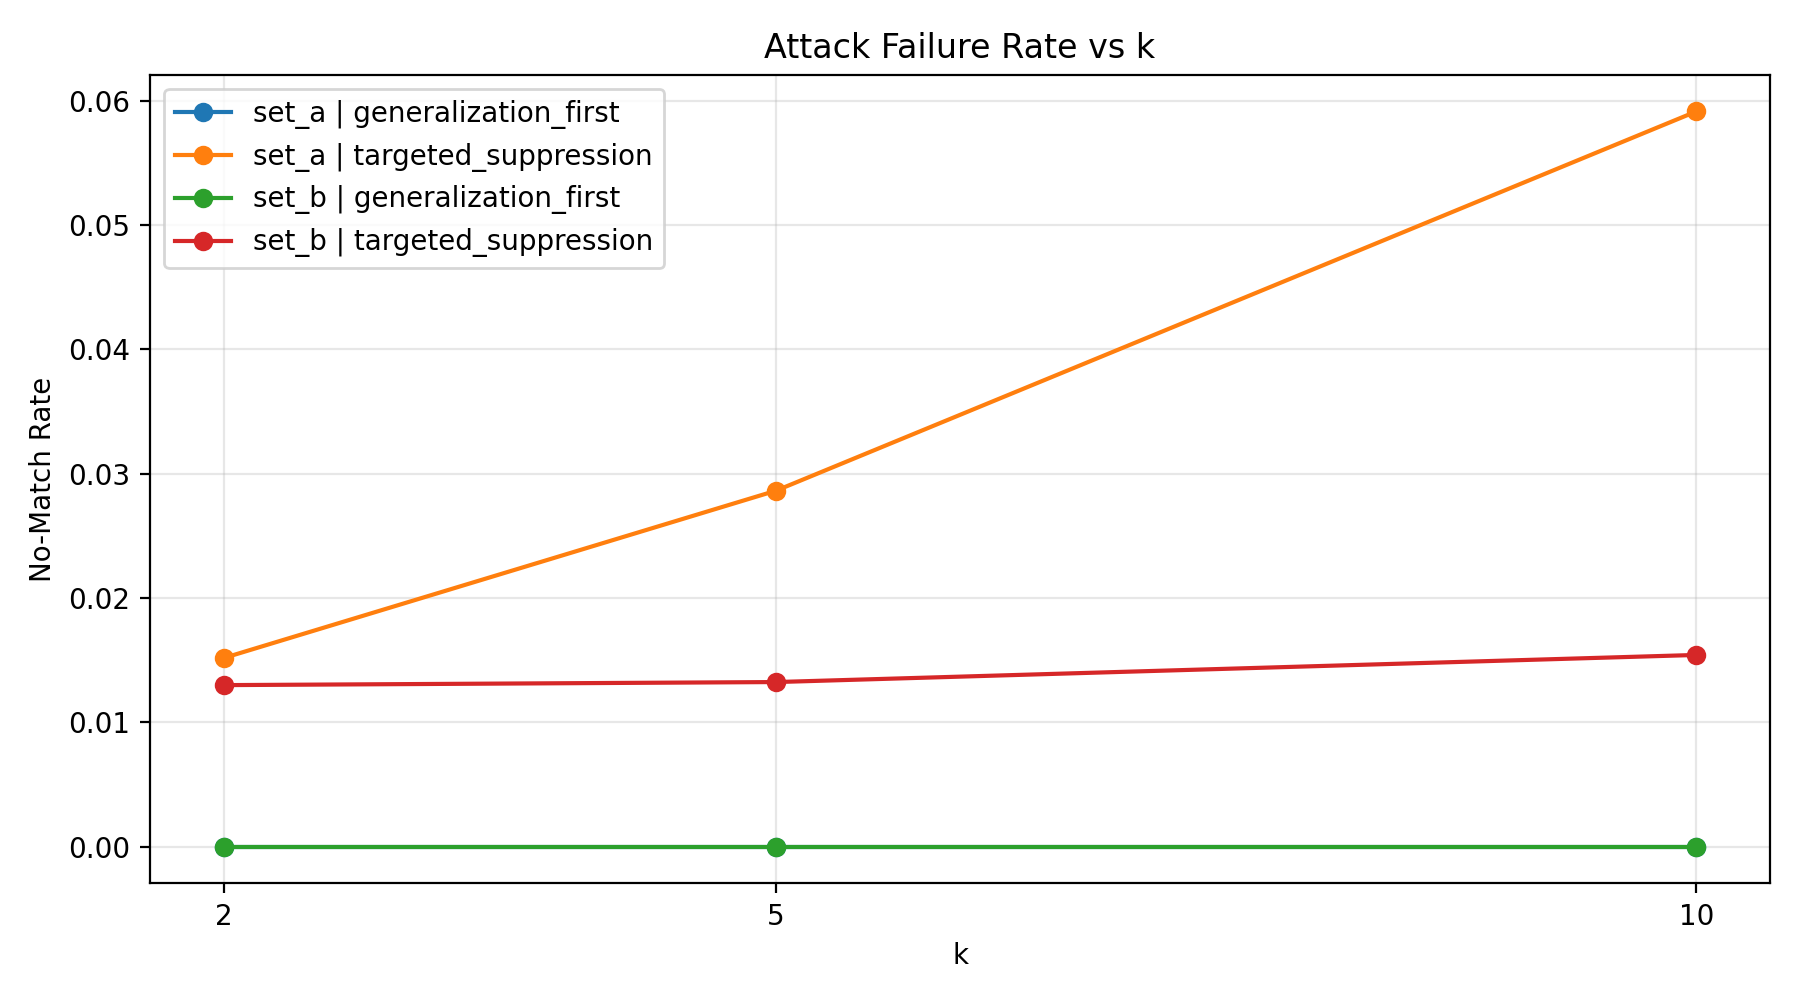
\includegraphics[width=0.92\textwidth]{risk_vs_k.png}
\end{frame}

\begin{frame}{Utility Loss vs k}
    \centering
    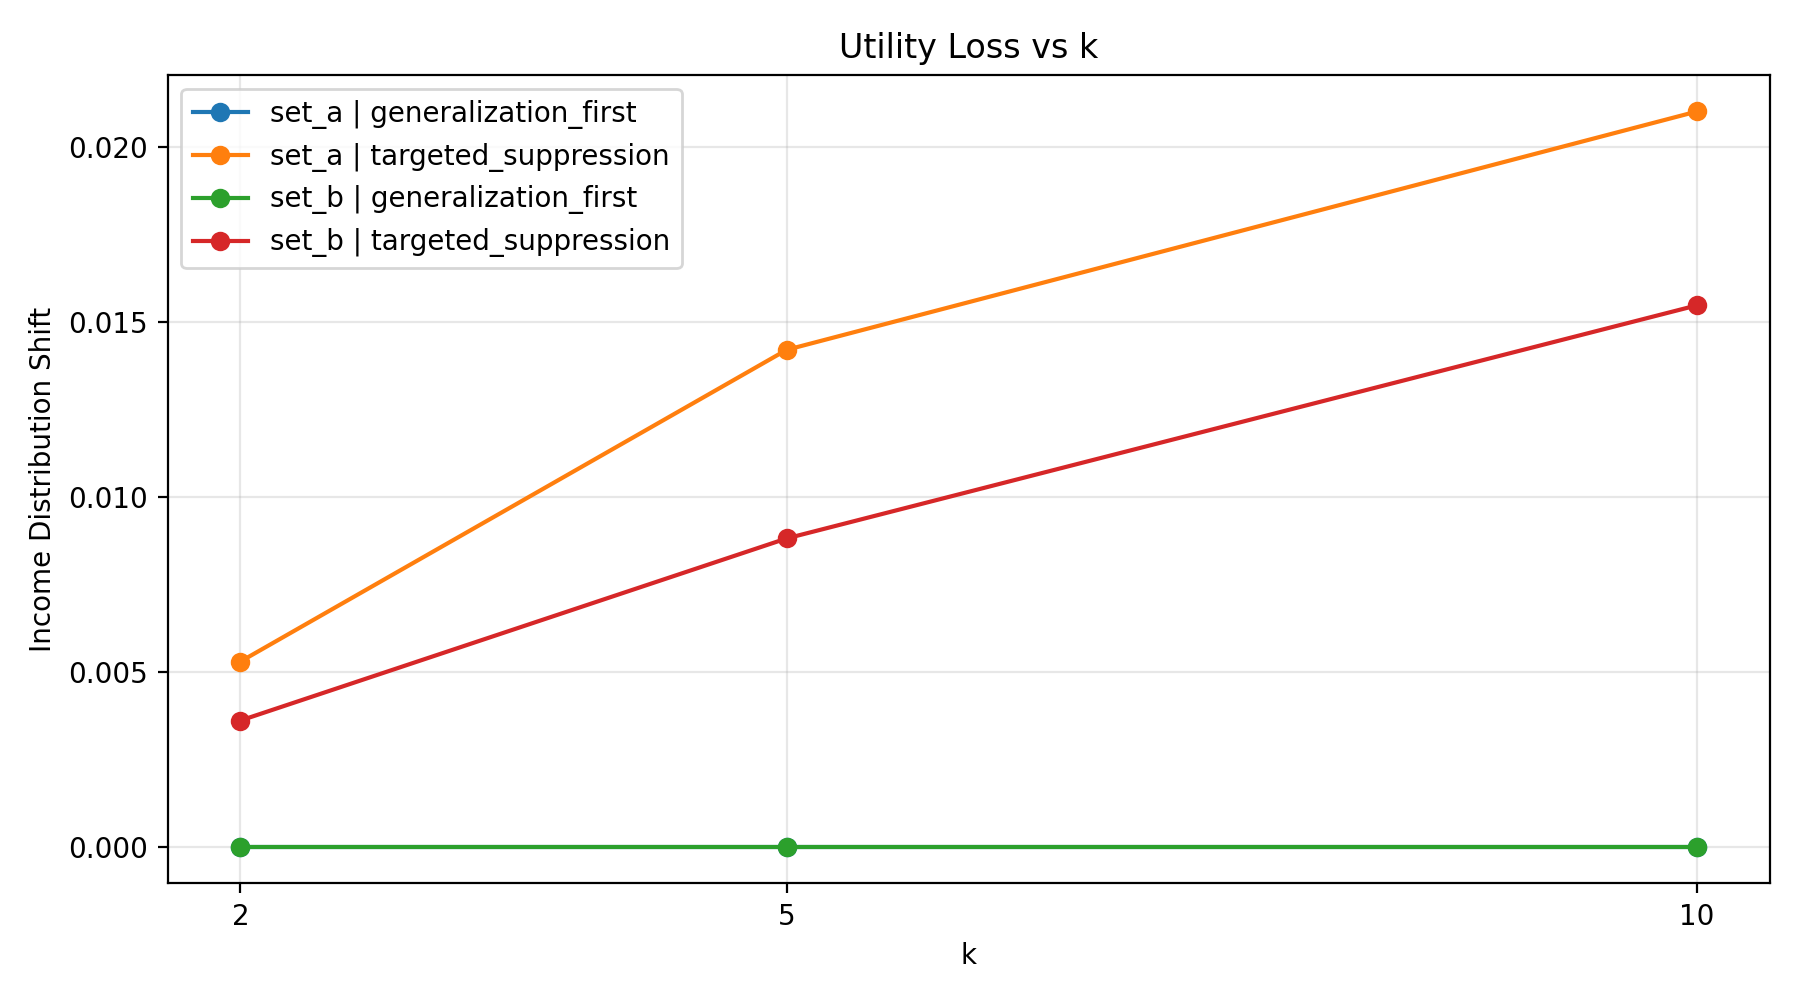
\includegraphics[width=0.92\textwidth]{utility_vs_k.png}
\end{frame}

\begin{frame}{Key Results}
    \begin{itemize}
        \item Generalization-first keeps all rows but has very high information loss.
        \item Targeted suppression keeps 94.0\% to 98.7\% of rows depending on the setup.
        \item QI Set A with targeted suppression at $k=2$ gives the best balance in this implementation.
        \item Stronger privacy increases attack failure, but also increases information loss.
    \end{itemize}
\end{frame}

\begin{frame}{Example Comparison}
    \centering
    \small
    \begin{tabular}{lrrrr}
        \toprule
        Setup & Retention & No-Match & Info Loss & Income Shift \\
        \midrule
        Set A, TS, $k=2$ & 98.6\% & 1.5\% & 0.076 & 0.0014 \\
        Set A, TS, $k=10$ & 94.0\% & 5.9\% & 0.177 & 0.0065 \\
        Set B, TS, $k=2$ & 98.7\% & 1.3\% & 0.157 & 0.0004 \\
        Set B, GF, $k=10$ & 100.0\% & 0.0\% & 0.917 & 0.0000 \\
        \bottomrule
    \end{tabular}
\end{frame}

\begin{frame}{Limitations}
    \begin{itemize}
        \item This project evaluates only k-anonymity, not l-diversity or t-closeness.
        \item The attacker is simulated from the same source population.
        \item Utility is measured with lightweight descriptive metrics rather than full downstream tasks.
    \end{itemize}
\end{frame}

\begin{frame}{Conclusion}
    \begin{itemize}
        \item The project delivers a full k-anonymity workflow with validation and reporting.
        \item Exact unique linkage can be eliminated, but the privacy--utility trade-off remains central.
        \item The most practical release in this implementation is QI Set A with targeted suppression at low $k$.
    \end{itemize}
\end{frame}

\begin{frame}{Demo Flow}
    \begin{itemize}
        \item Open the repository and show the dataset structure.
        \item Run \texttt{python scripts/run\_experiments.py}.
        \item Show \texttt{results/metrics/experiment\_summary.csv}.
        \item Show the two generated plots.
        \item Open the final report PDF.
    \end{itemize}
\end{frame}

\end{document}
